\chapter{Simulation Results}
\section{DC Analysis}
\begin{figure} [H]
\centering
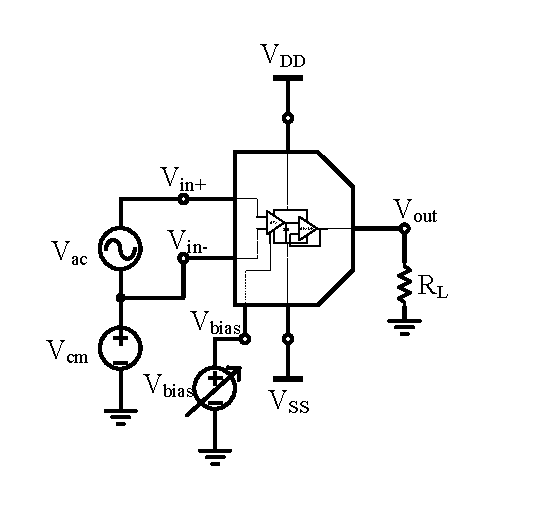
\includegraphics[scale=1]{Figures/Test_Benches/Overall/ACDC.pdf}
\caption{Test setup for DC Analysis}
\end{figure}



\section{AC Analysis}

\begin{figure} [H]
\centering
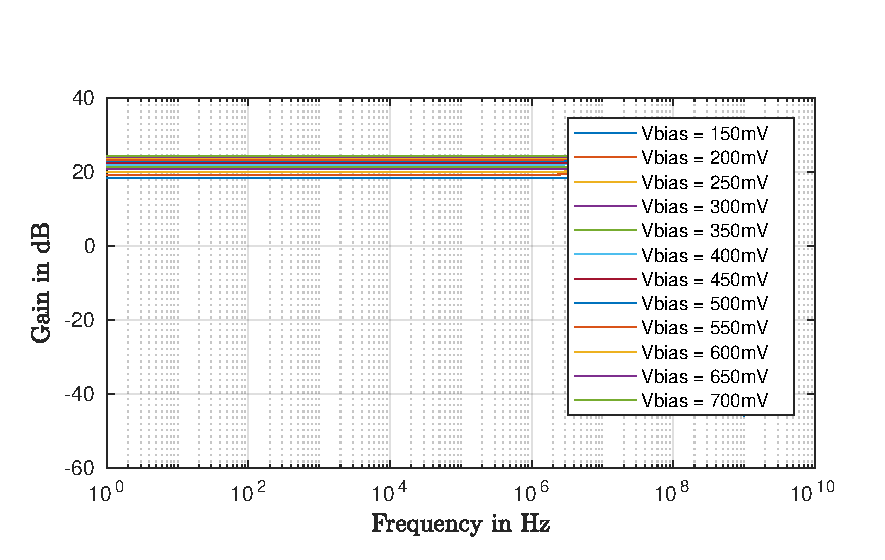
\includegraphics[scale=1]{Figures/Plots/Ov_Gain.pdf}
\caption{Plot of Gain vs Frequency for different Vbias}
\end{figure}

\begin{figure} [H]
\centering
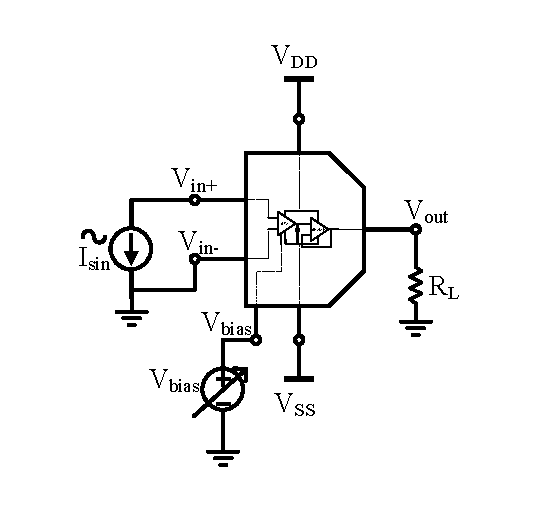
\includegraphics[scale=1]{Figures/Test_Benches/Overall/ZIN.pdf}
\caption{Test setup to measure Input Impedance}
\end{figure}

\begin{figure} [H]
\centering
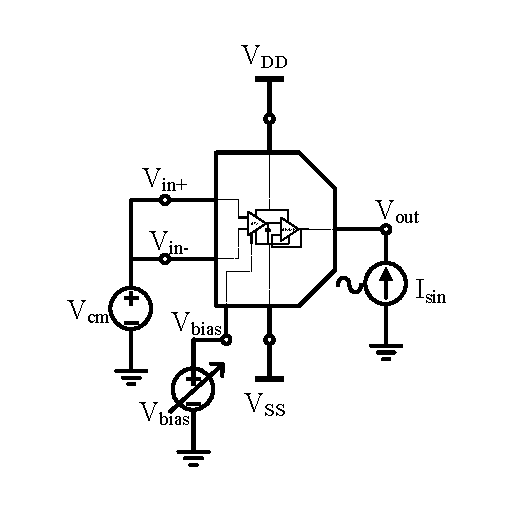
\includegraphics[scale=1]{Figures/Test_Benches/Overall/ZOUT.pdf}
\caption{Test setup to measure Output Impedance}
\end{figure}

\begin{figure} [H]
\centering
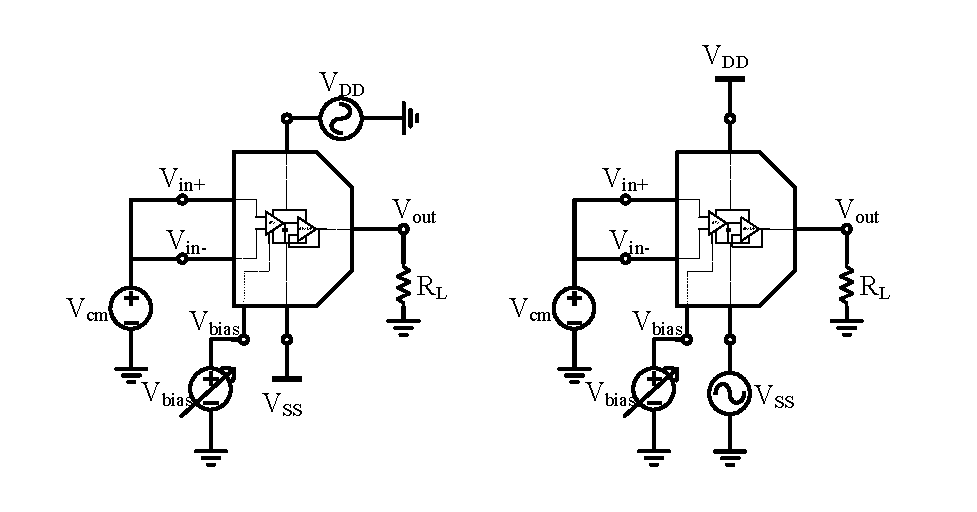
\includegraphics[scale=1]{Figures/Test_Benches/Overall/PSRR.pdf}
\caption{Test setup to measure PSRR}
\end{figure}

\section{Transient Analysis}
\begin{figure} [H]
\centering
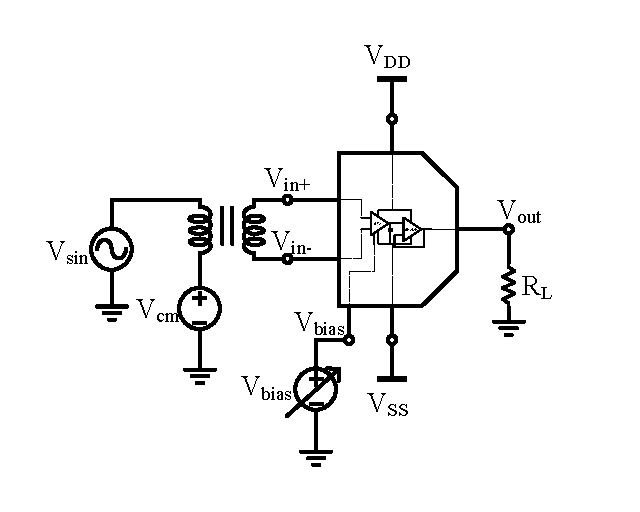
\includegraphics[scale=1]{Figures/Test_Benches/Overall/SINE.pdf}
\caption{Test setup for Transient Analysis - Sine Wave input}
\end{figure}

\begin{figure} [H]
\centering
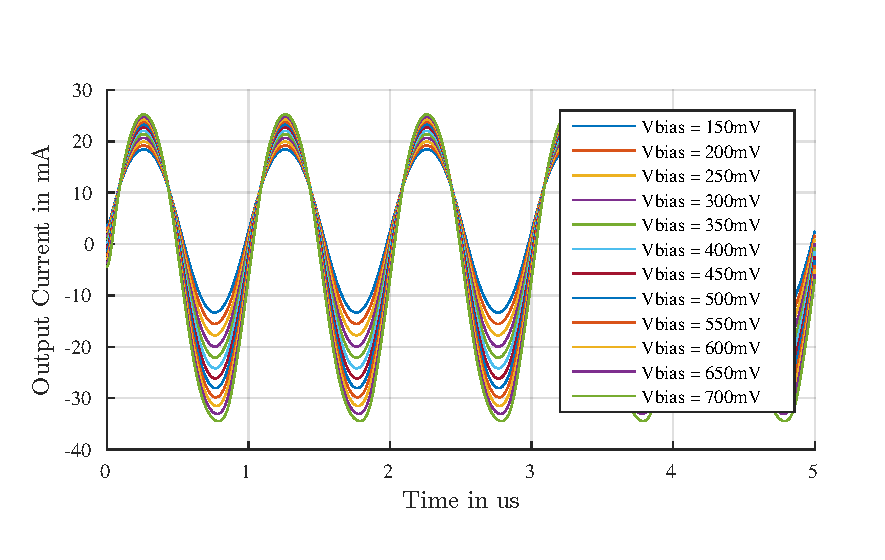
\includegraphics[scale=1]{Figures/Plots/Ov_Sine_Iout.pdf}
\caption{Plot of Output Current vs time for different Vbias}
\end{figure}

\begin{figure} [H]
\centering
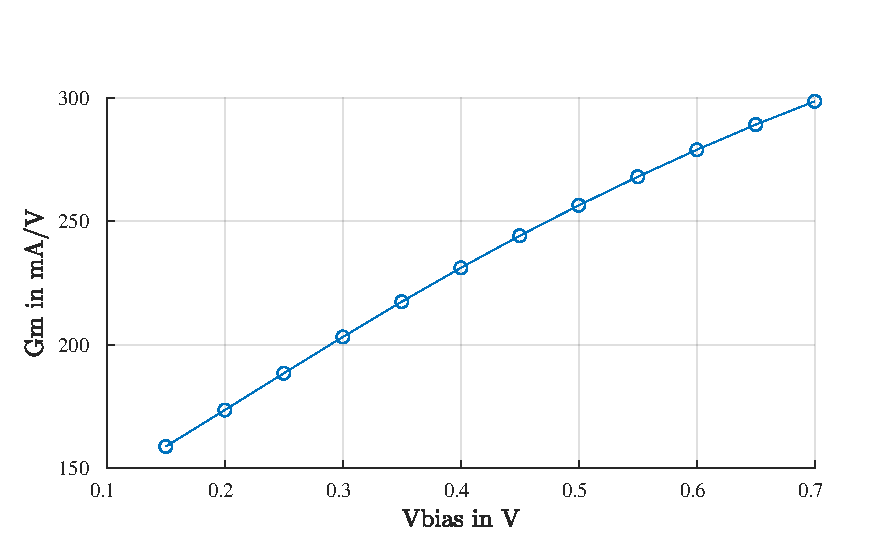
\includegraphics[scale=1]{Figures/Plots/Ov_Gm.pdf}
\caption{Plot of Gm vs Vbias}
\end{figure}

\begin{figure} [H]
\centering
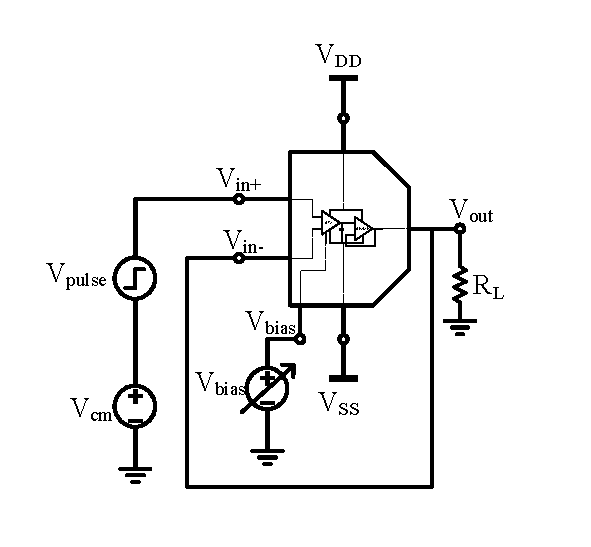
\includegraphics[scale=1]{Figures/Test_Benches/Overall/SLEW.pdf}
\caption{Test setup for Transient Analysis - Square Wave input}
\end{figure}

\section{Noise Analysis}

\begin{figure} [H]
\centering
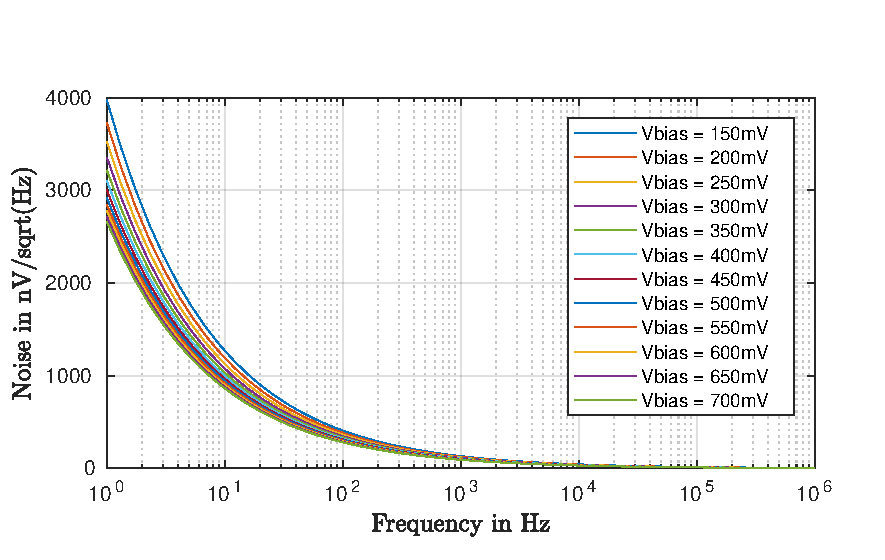
\includegraphics[scale=1]{Figures/Plots/Ov_Noise.pdf}
\caption{Plot of Input Referred Noise vs Frequency for different Vbias}
\end{figure}

\section{Pragrammable Load}

\begin{figure} [H]
\centering
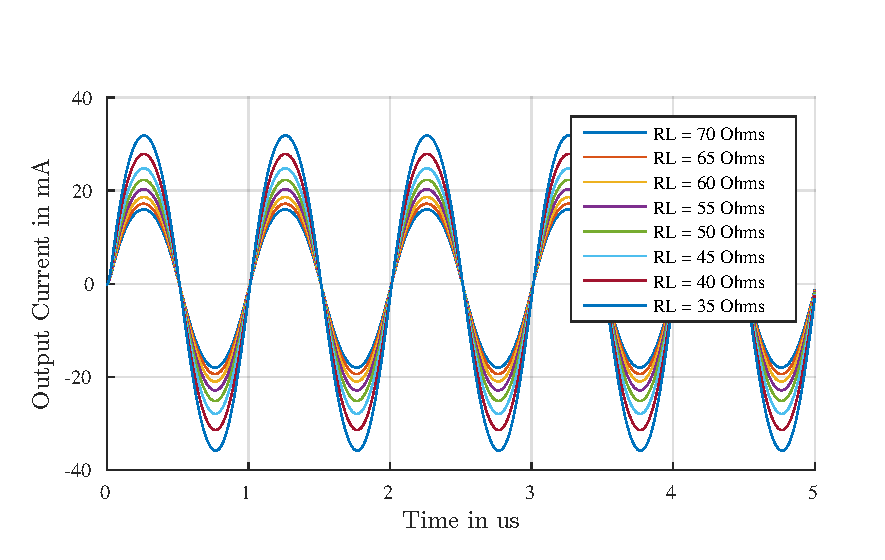
\includegraphics[scale=1]{Figures/Plots/Ov_Sine_RL.pdf}
\caption{Plot of Output Current vs Time for different RL}
\end{figure}

\begin{figure} [H]
\centering
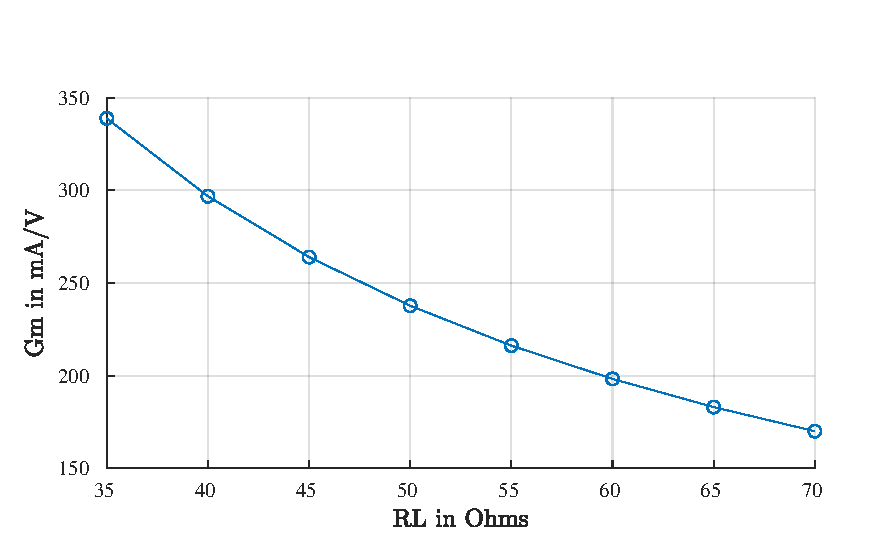
\includegraphics[scale=1]{Figures/Plots/Ov_Gm_RL.pdf}
\caption{Plot of Output Current vs time for different RL}
\end{figure}

\section{Corner Simulation}
\subsection{Process Variation}
\subsection{Process and Supply Variation}
\subsection{Process, Voltage and Temperature (PVT) variation}
\subsection{Summary of PVT Corner Analysis}